\section{Personalized Fast FullSubNet}

\subsection{Motivation}

The Fast FullSubNet (FFSN) model \cite{hao2023fast} offers a lightweight and efficient subband-based speech enhancement model that maintains high performance in noise reduction tasks.
However, the model was not designed for personalized speech enhancement.
To introduce personalization, we propose a personalized Fast FullSubNet (PFFSN) model leveraging the model's ability to process subbands. PFFSN consists of two major modules: a speaker embedding module and a denoising module.
The speaker embedding module is responsible for extracting speaker-specific features from the input speech signal, while the denoising module is responsible for enhancing the speech signal based on the extracted speaker features.
The architecture of the PFFSN model is shown in Figure \ref{fig:pffsn-arch}.

\begin{figure}[H]
    \centering
    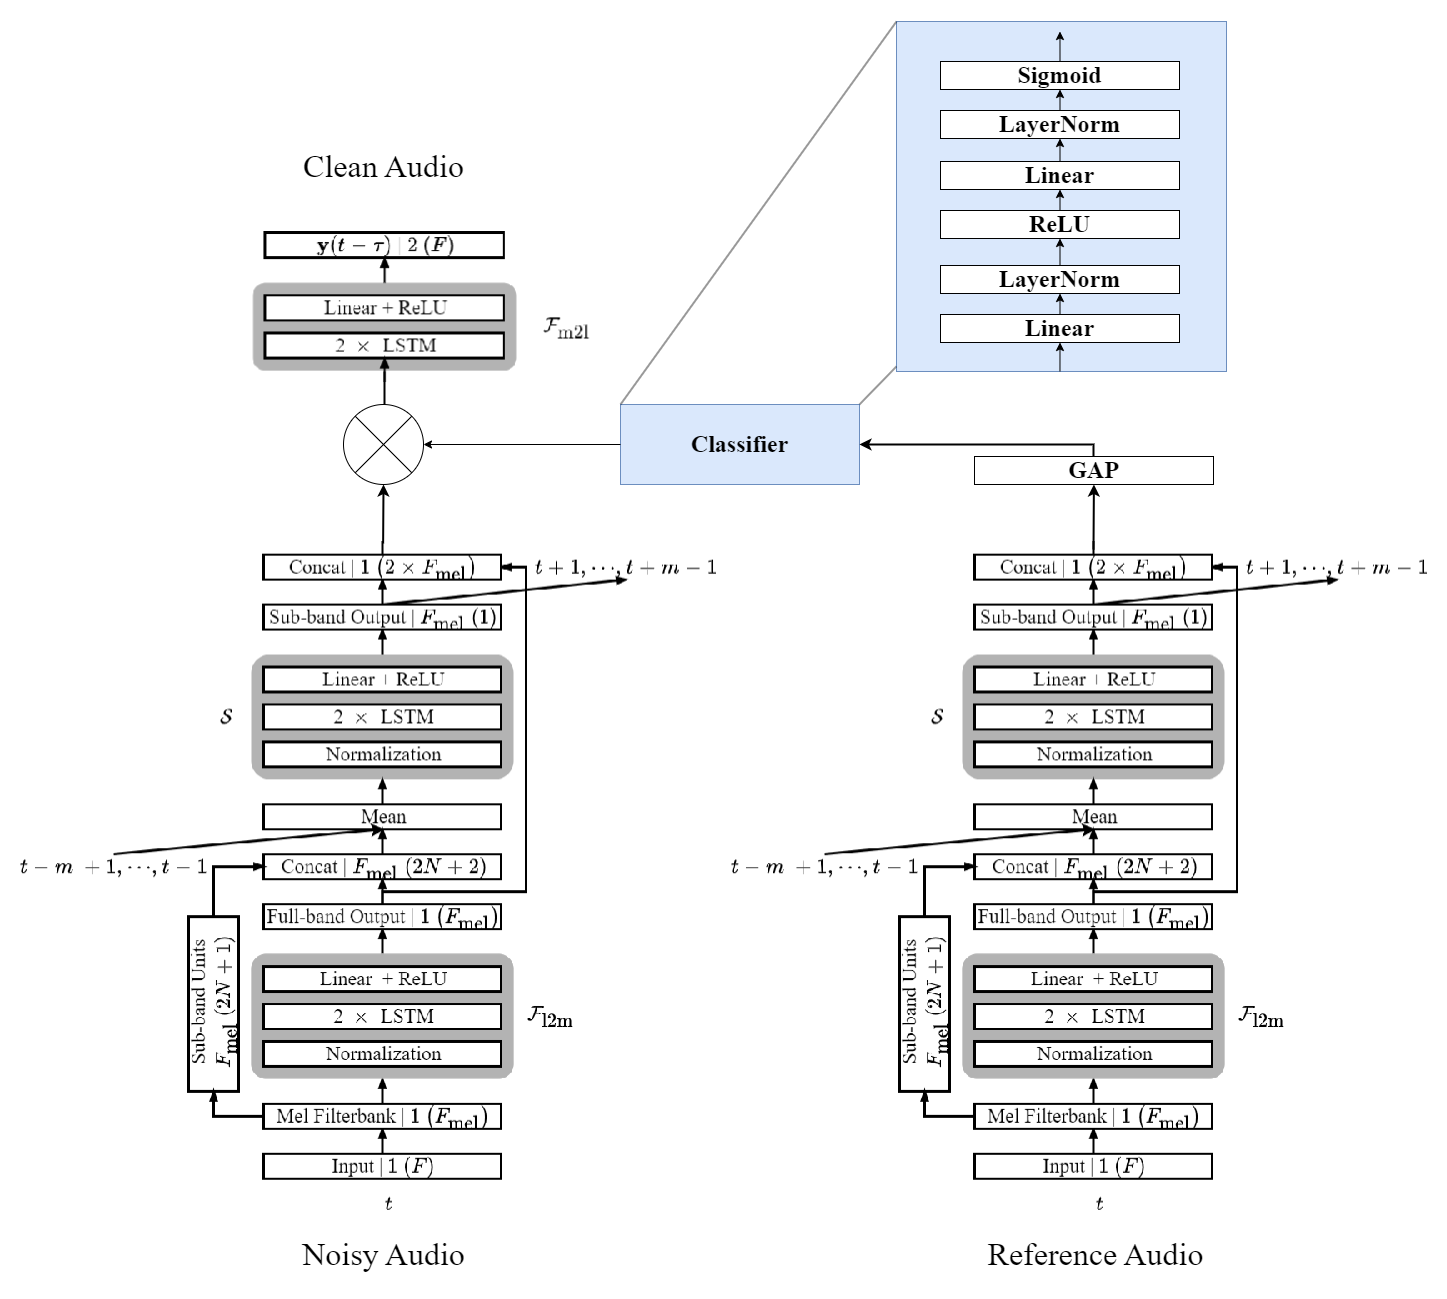
\includegraphics[width=0.8\textwidth]{images/experiments/pffsn/pffsn-arch.png}
    \caption{PFFSN model architecture}
    \label{fig:pffsn-arch}
\end{figure}

\subsection{Speaker Embedding Module}
The speaker embedding module consists of the encoder and bottleneck layers of FFSN followed by a simple feedforward network.
The encoder and bottleneck layers are responsible for extracting subband features of the speaker given a clean speech signal.
The feedforward network aims to classify whether the targeted speaker voice resides in a subband or not.
The feedforward network consists of two fully connected layers with LayerNorms and ReLU activation functions and a sigmoid activation function in the output layer.
The output of the sigmoid activation is the probability of the speaker's voice residing in the subband.

\subsection{Denoising Module}
The denoising module is a regular FFSN model in which its decoder input subbands are scaled based on the speaker embedding module's output.
Subbands in which the speaker's voice is detected are amplified, while the others are suppressed.
This process aims to help the decoder focus on enhancing the speaker's voice while suppressing the noise.


\subsection{Experimental Setup}

We trained the PFFSN model on the training set of our dataset for 43 epochs with a batch size of 16 per GPU. We trained the model using Kaggle's 2 NVIDIA Tesla T4 GPUs.
The noisy audio clips were generated on the fly by mixing speakerA and speakerB clean audio clips. The SNR of the noisy audio clips was randomly selected from values of 0, 3, 6, 10, 20.
The clean audio clips were cropped to 3 seconds before mixing as an augmentation technique. The audio clips were sampled at 16kHz.
The Adam optimizer was used with a learning rate of $5 \times 10^{-5}$ with Cosine Annealing and beta values of 0.9 and 0.999. Model exponential moving average (EMA) was used with a decay of 0.999.
We employed a mixture of loss functions, including L1 loss, Multi-Resolution STFT loss, complex Ration Mask (cRM) loss, and TAP loss with weights 1, 0.5, 1, and 0.3 respectively.
The weights of the Speaker Embedding Module and Denoising Module were initialized using weights from an FFSN model trained on DNS 2021 data to overcome limited data availability.
Figure \ref{fig:pffsn-loss} shows the training loss curve of the PFFSN model.

%% add subfigures for 5 losses curves
\begin{figure}[H]
    \centering
    \begin{subfigure}{0.49\textwidth}
        \centering
        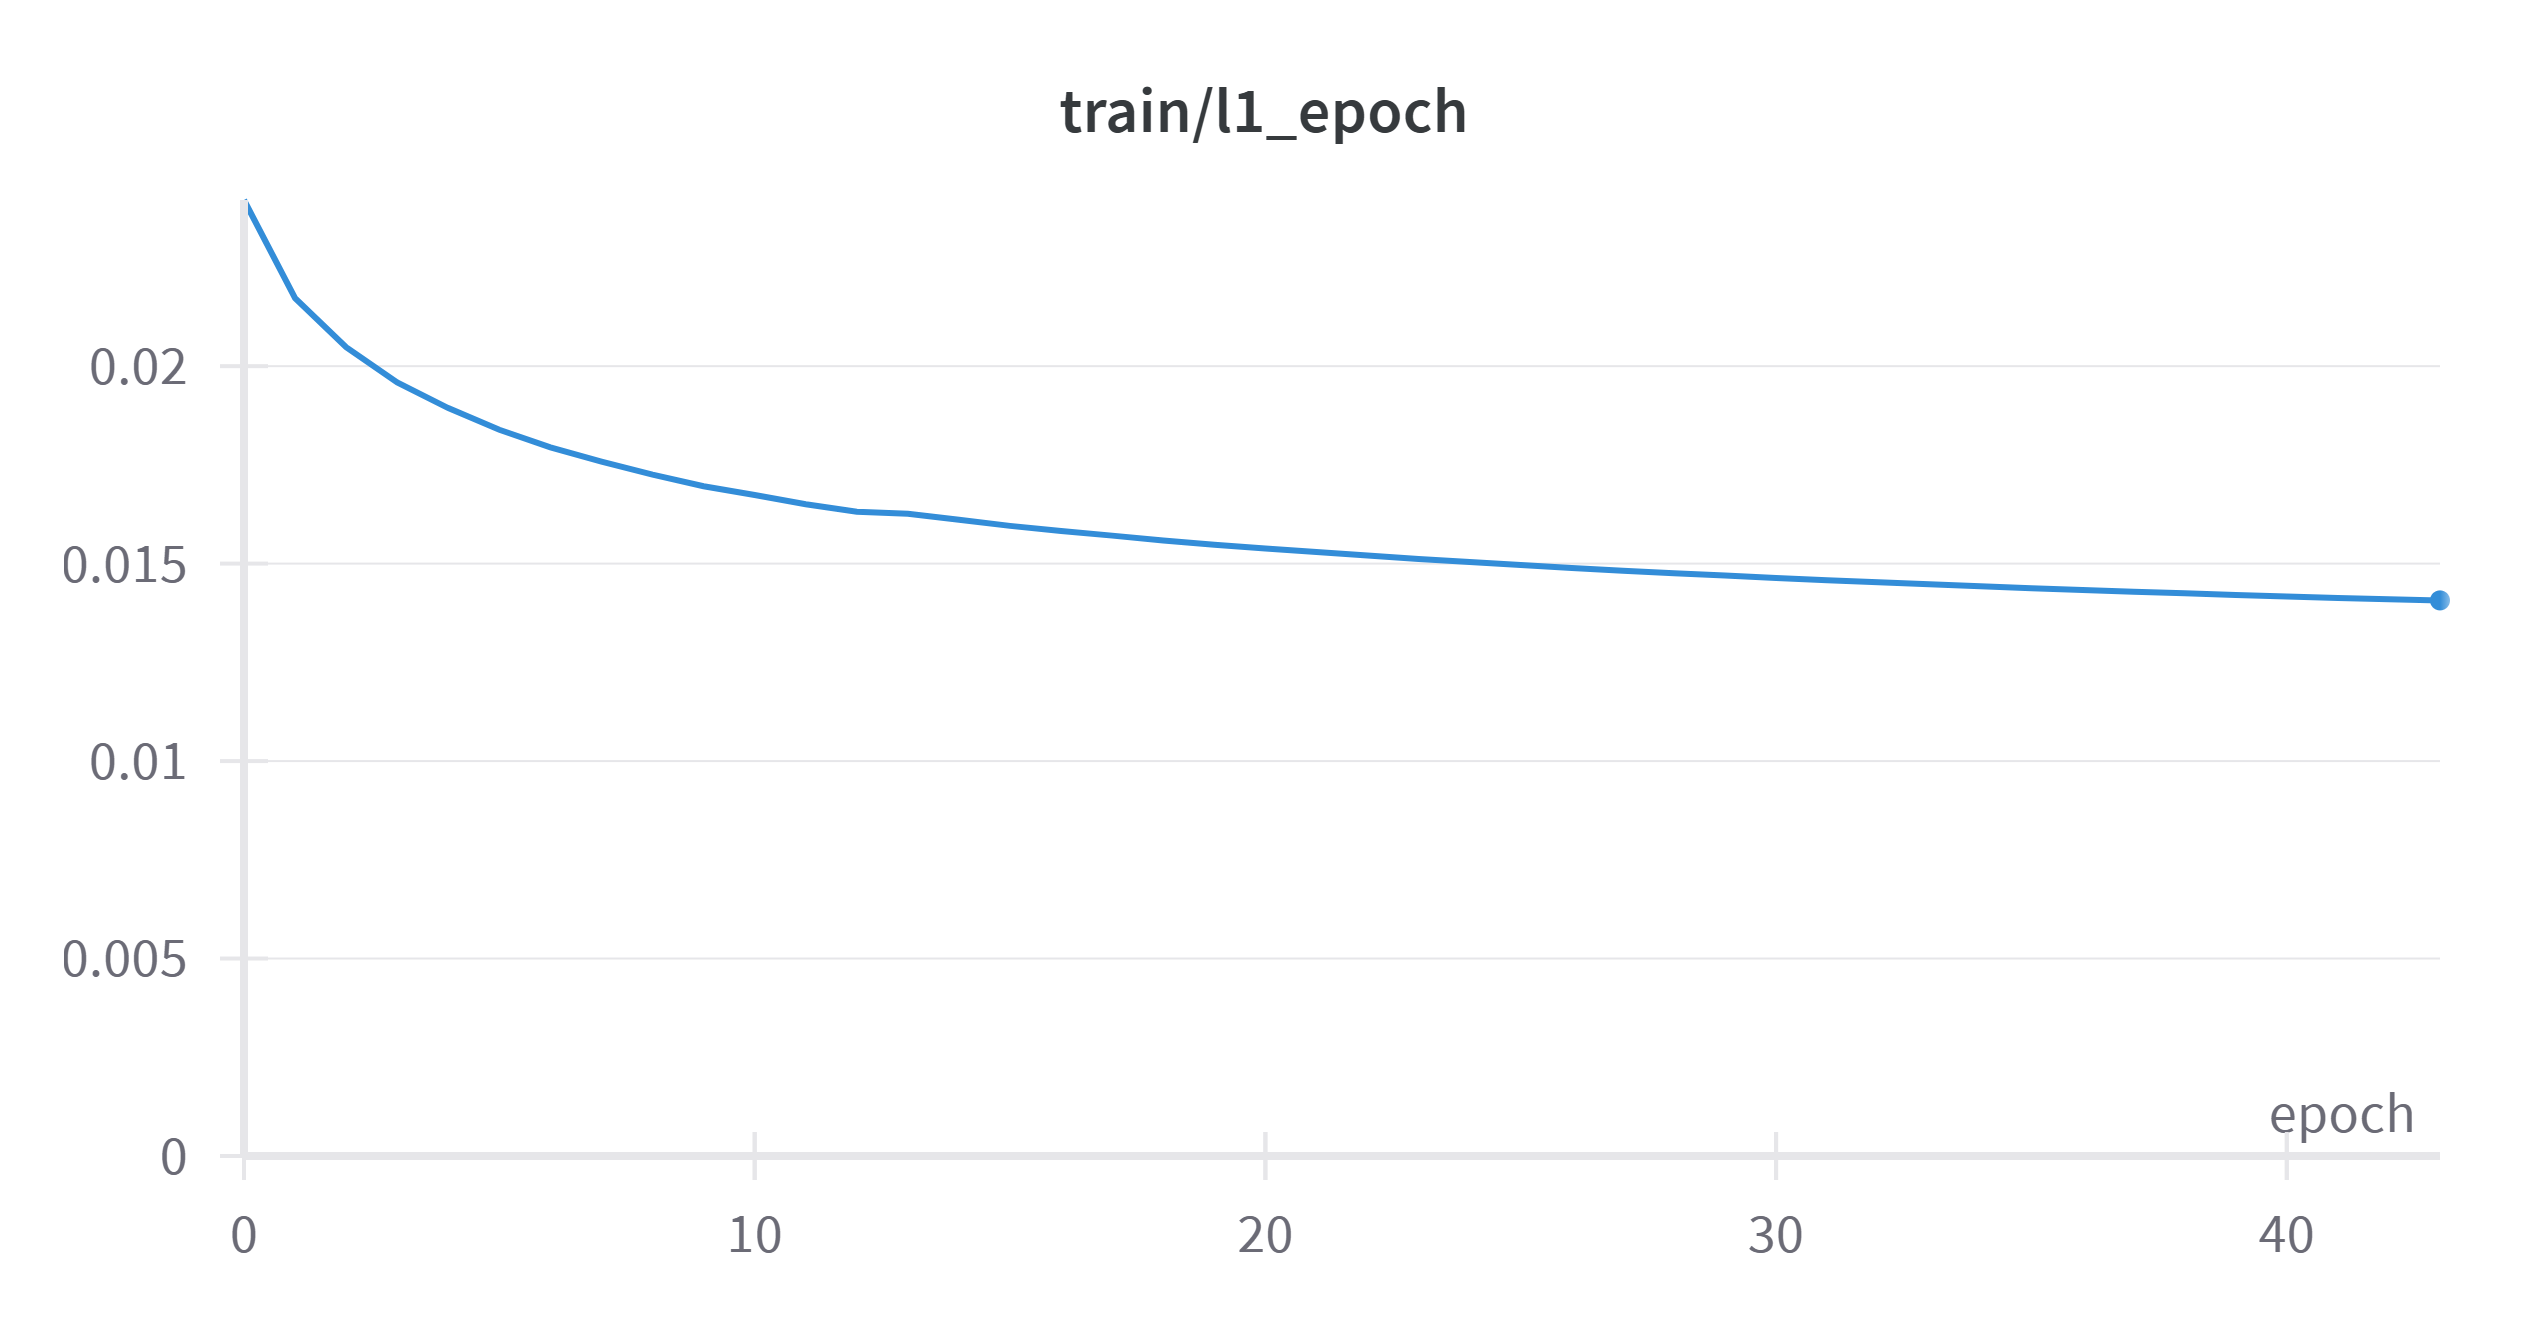
\includegraphics[width=\textwidth]{images/experiments/pffsn/train_l1.png}
        \caption{L1 Loss}
    \end{subfigure}
    \begin{subfigure}{0.49\textwidth}
        \centering
        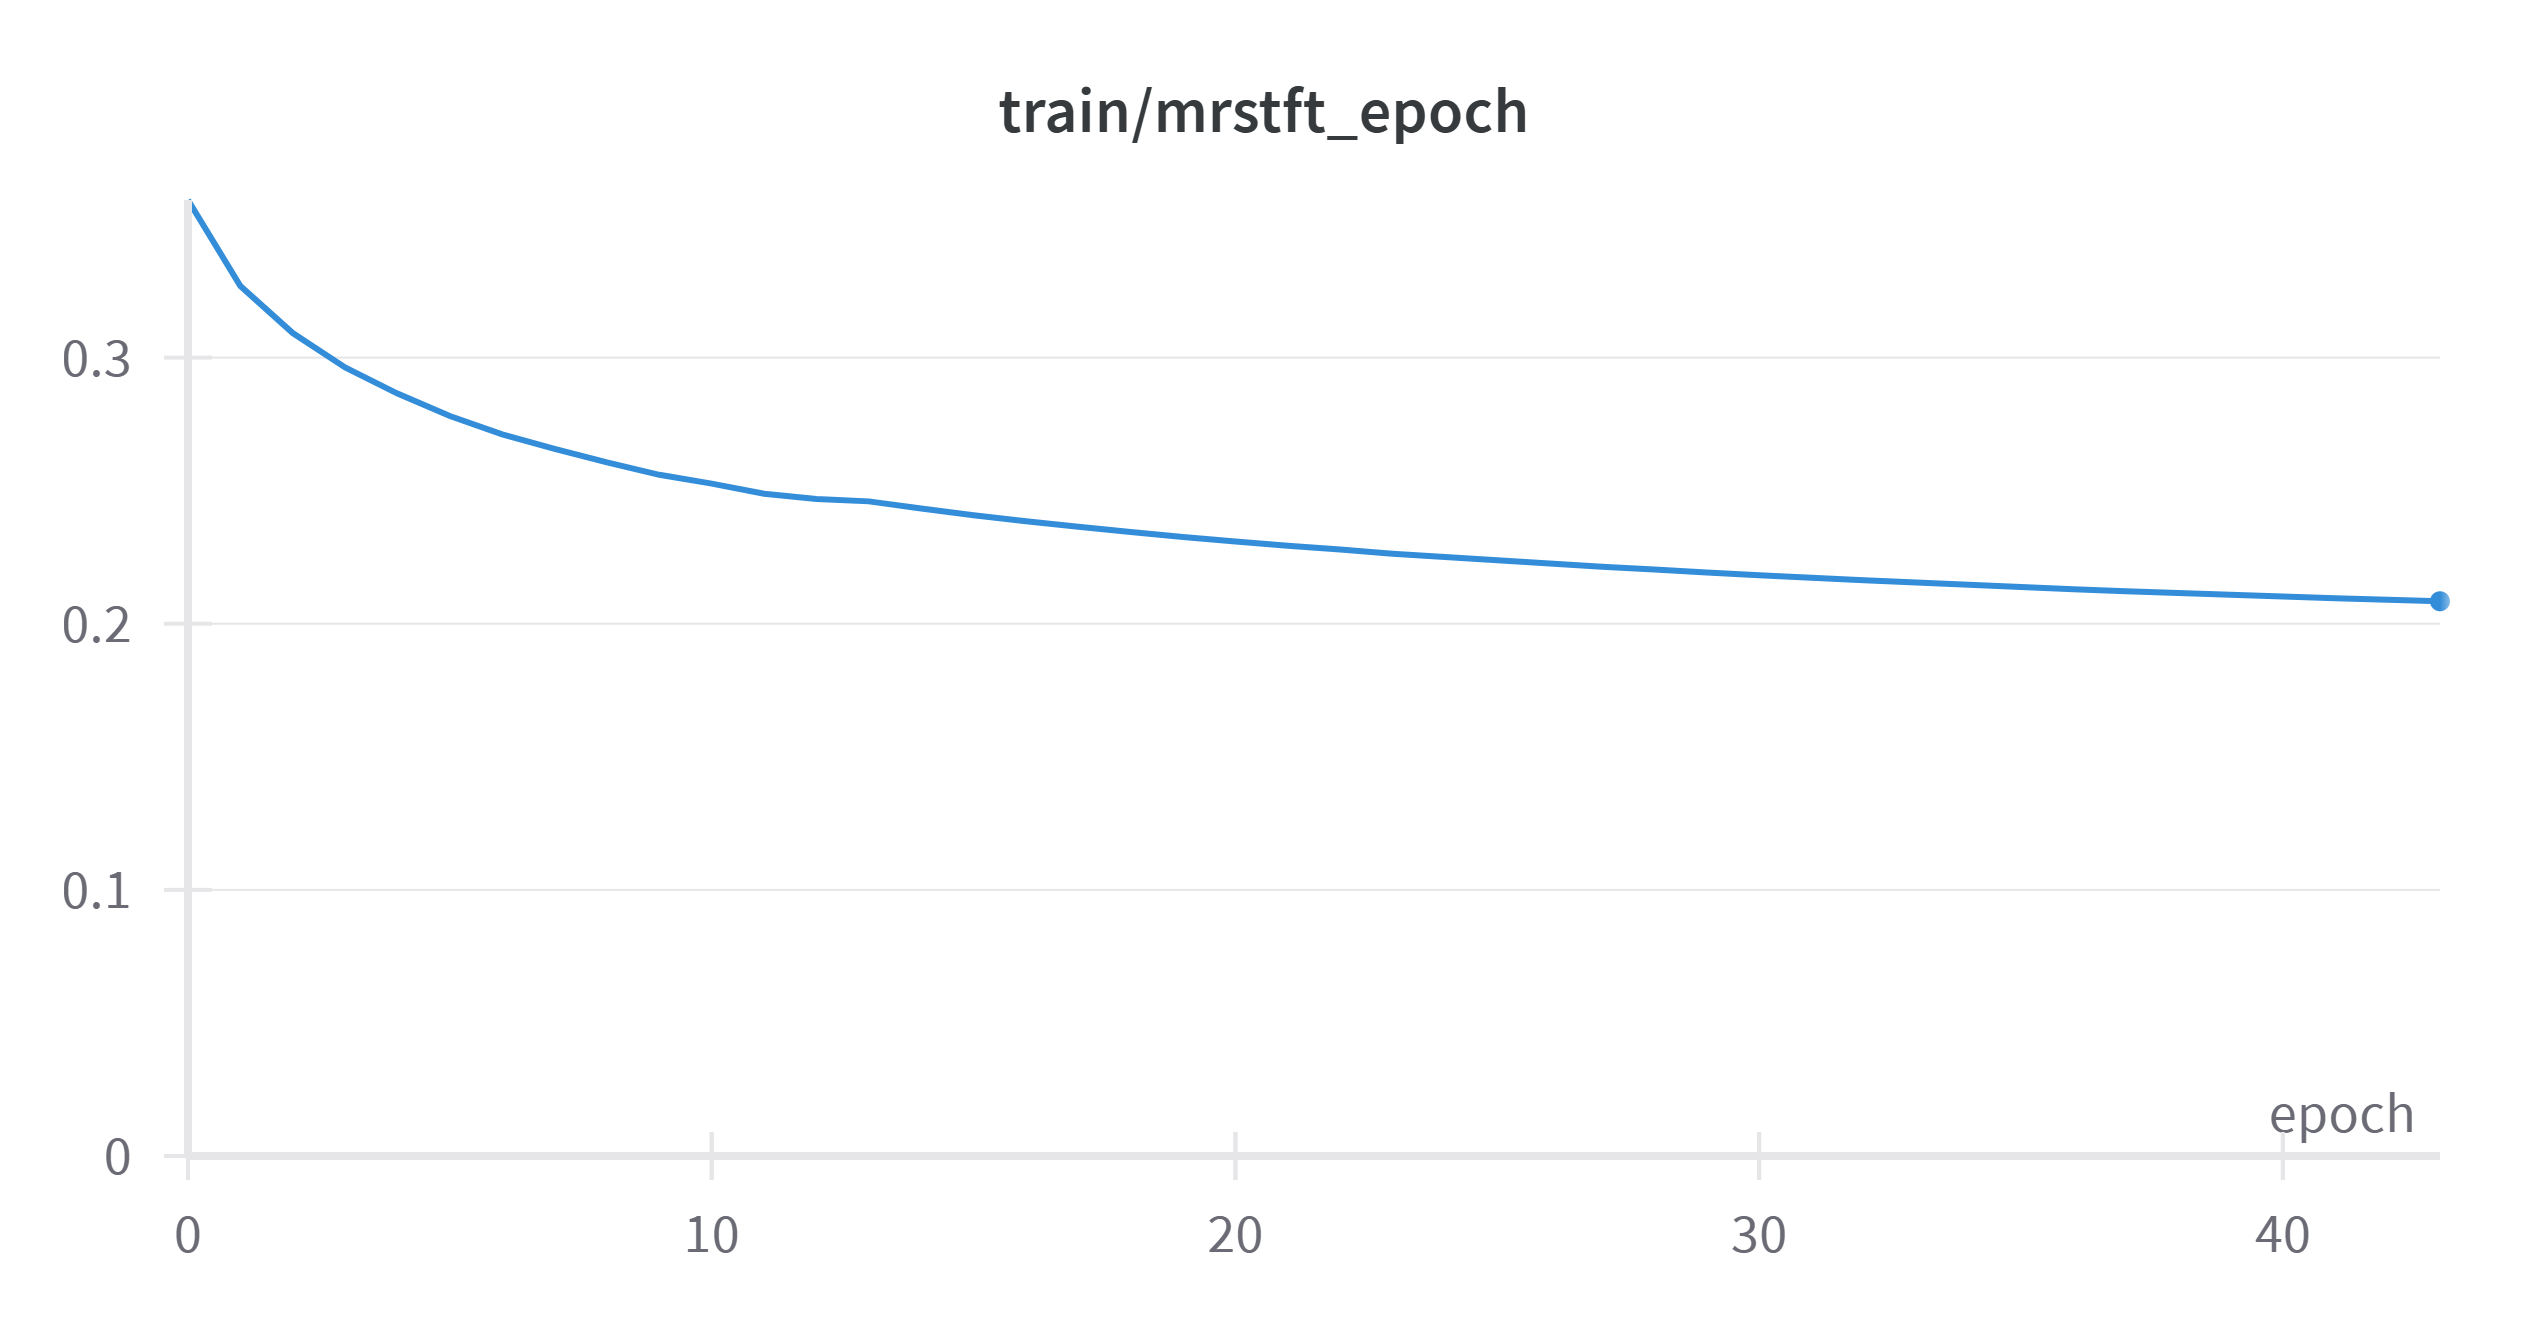
\includegraphics[width=\textwidth]{images/experiments/pffsn/train_mrstft.png}
        \caption{Multi-Resolution STFT Loss}
    \end{subfigure}
    \begin{subfigure}{0.49\textwidth}
        \centering
        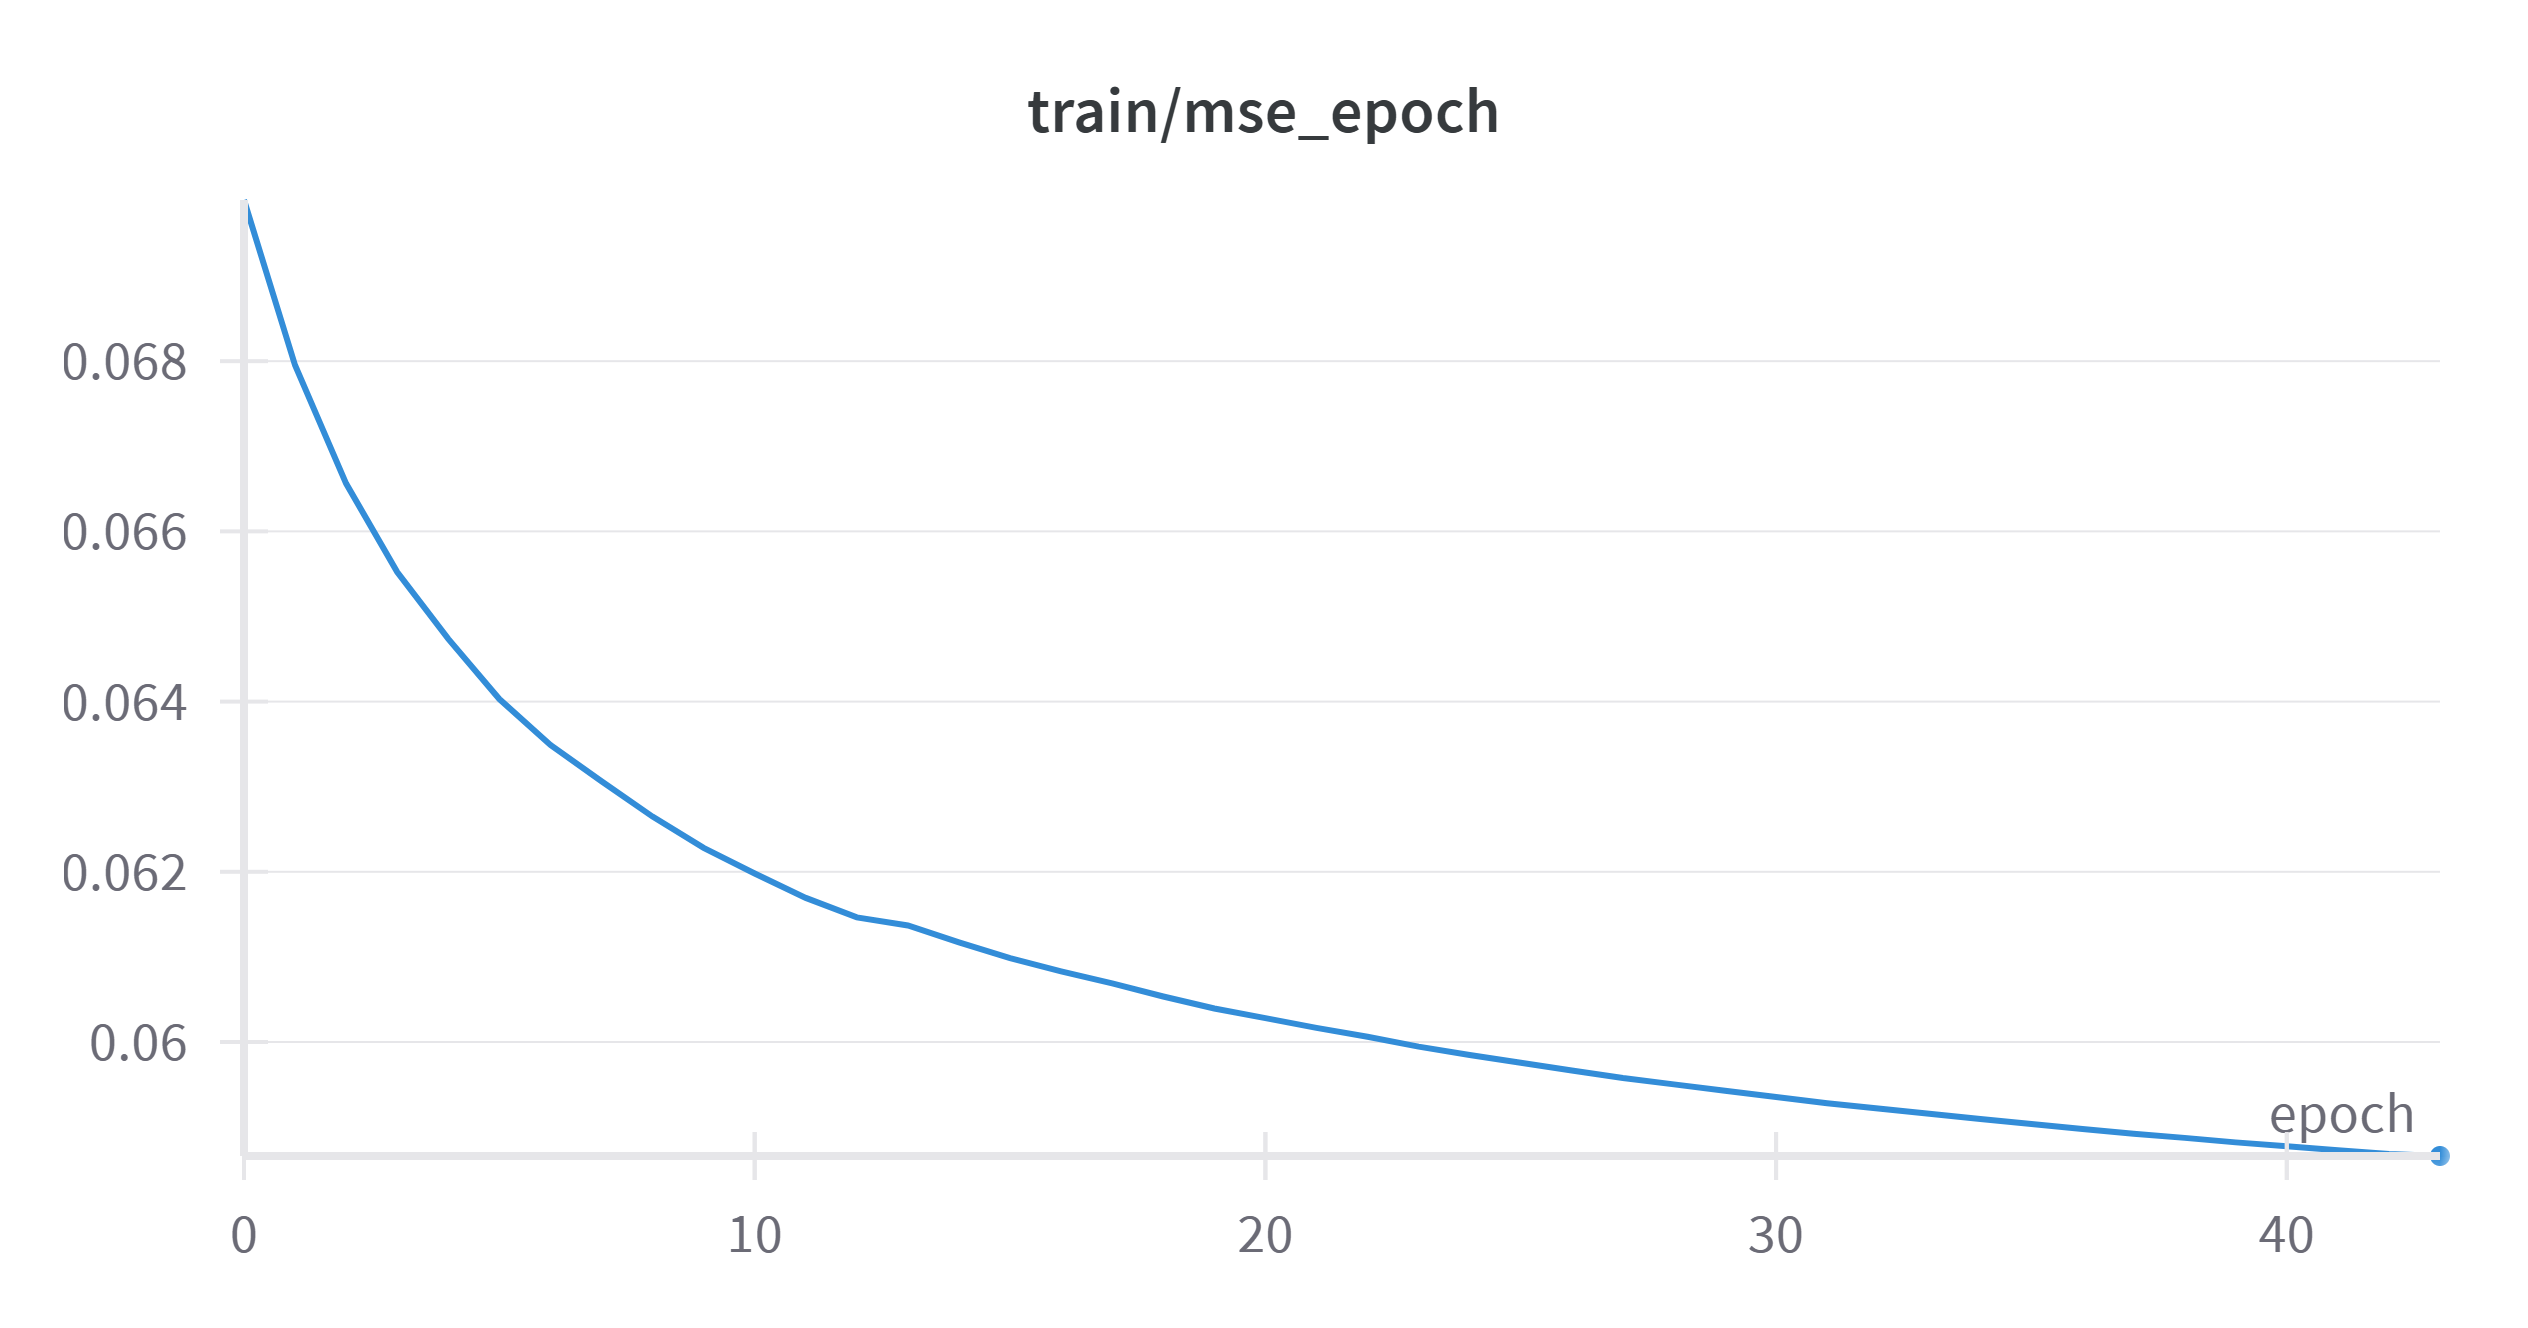
\includegraphics[width=\textwidth]{images/experiments/pffsn/train_cRM.png}
        \caption{Complex Ratio Mask Loss}
    \end{subfigure}
    \begin{subfigure}{0.49\textwidth}
        \centering
        
\includegraphics[width=\textwidth]{images/experiments/pffsn/train_tap_loss.png}
        \caption{TAP Loss}
    \end{subfigure}
    \caption{PFFSN model training loss curves}
    \label{fig:pffsn-loss}
\end{figure}

\subsection{Results}
We tested the model on two test sets: a personalized DNS blind test set and the test set of our dataset. Results are shown in table \ref{tab:pffsn-results}.

\begin{table}[]
    \centering
    \begin{tabular}{ccccccc}
        \hline
        \multirow{2}{*}{Metric} & \multicolumn{5}{c}{Collected DataSet (Different SNR)} & \multirow{2}{*}{\begin{tabular}[c]{@{}c@{}}Personalized DNS\\ Blind set\end{tabular}}                                 \\ %%\cline{2-6}
                                & 0                                                     & 3                                                                                     & 6     & 10    & 20    &       \\ \hline
        DNSMOS/SIG              & 3.291                                                 & 3.312                                                                                 & 3.362 & 3.533 & 3.781 & 3.524 \\
        DNSMOS/BAK              & 1.848                                                 & 2.004                                                                                 & 2.252 & 2.661 & 3.393 & 2.824 \\
        DNSMOS/OVRL             & 1.963                                                 & 2.080                                                                                 & 2.263 & 2.587 & 3.113 & 2.518 \\
        PESQ nb                & 1.468                                                 & 1.741                                                                                 & 2.075 & 2.512 & 3.253 & -     \\
        PESQ wb                & 1.205                                                 & 1.380                                                                                 & 1.654 & 2.086 & 2.927 & -     \\
        STOI                    & 0.717                                                 & 0.804                                                                                 & 0.866 & 0.916 & 0.955 & -     \\ \cline{1-7}
    \end{tabular}
    \caption{PFFSN model results on the collected dataset test set using different SNR levels and on the personalized DNS blind test set}
    \label{tab:pffsn-results}
\end{table}


\subsection{Limitations}
After listening to some outputs, one can notice that the performance of the model degrades when the tones of the voice in the input change frequently.
This is due that the model follows the subband approach that focuses on the removal of stationary noises.
One can also notice that the model performs well when the interfering voice or noises reside in frequency ranges different from the ones where the main voice lies e.g., male and female interference,
due to the ease of subband classification. On the other hand, the model finds hard times when the voices are in the same ranges e.g., male and male interference.
Furthermore, low SNR audio clips are harder to enhance, low SNR audio might simulate scenarios where the two speakers are within the same proximity to the microphone which might not be the case in a teleconferencing scenario.